\section{Multidisciplinary Design Optimization MDO}
The multidisciplinary design optimization \textbf{MDO} is a field of engineering that uses optimization method in design problems incorporating an high number of disciplines. \\
Due to its multidisciplinary nature, aircraft design problems is one of the first application of the MDO.
Aerospace vehicles are extremely complex systems, and their design needs the detailed consideration of disciplines such as aerodynamics, structural mechanics, materials, control, propulsion, etc ... and the interacting between this disciplines.\\
The MDO thus makes it possible to perform a design process ( determinate the value of the design variables ) joined to an optimization process ( find the value of design variables to obtain the best value for the objective function under constraints) in view of the interaction of the different disciplines involved in the process.\\
<<The main motivation for using MDO is that the performance of a multidisciplinary system is driven not only by the performance of the individual disciplines but also by their interactions.>> \cite{mart}
\\
\begin{figure}[H]
	\centering
	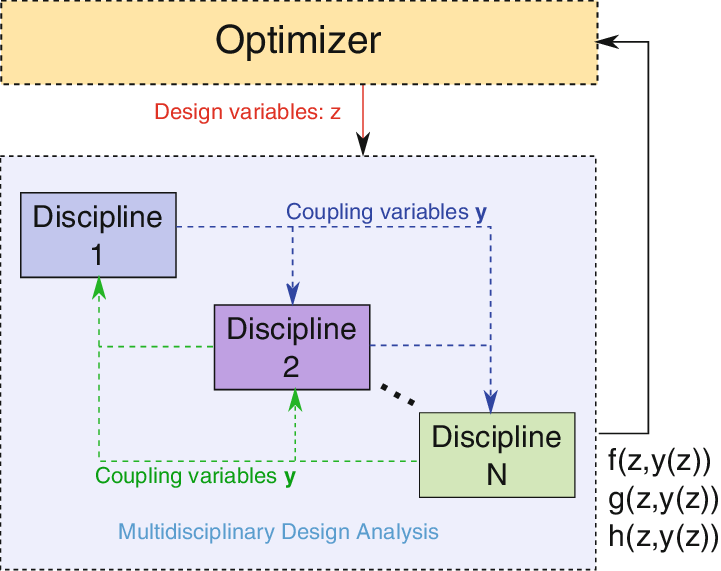
\includegraphics[width = .5\textwidth]{./Immagini/1_2.png}
	\caption{MDO scheme}
	\label{fig:1_1}
\end{figure}
Solving MDO problem in the early phase of the design process, by the support of advanced computational analysis tools, can improve the design and provide reduction of time and cost of the design cycle.\\
One of the first applications of the MDO was aircraft wing design, where there is a strong coupling between aerodynamics and structures, the aeroelastic coupling. After the application of MDO have been extended to the complete aircraft and to other field.\\
In MDO is important to define the architecture of the process,how organize the optimization software, the disciplines and the analysis of the model and the approximation model. So can be distinct two different architecture, the monolithic and the distributed. In the monolithic approach just one optimization problem will be solved, instead in the distributed approach there re multiple subproblem, which contain less variables and constraint, so the reaserch of the optimum of the main problem is split in the solving of little problems. So to solve the same optimal design problem there are many ways, and the choise of the architecture entails the computational cost and the final optimum design.

\subsection{Optimization Methods}

Computational design procedures are based on numerical analysis methods that evaluate the relative merit of a set of feasible designs. The merit of a design is based on the value of an objective function that is computed using numerical simulations such as CFD and CSM programs. The choice of objective function is extremely important and requires a deep knowledge of the multidisciplinary design problem at hand. \cite{mart2}
\\
A typical example of a constrained optimization problem can be represent as:

\begin{align*}
	&minimize \ \ F(x_i)\\
	&w.r.t. \ \ \ \ \ \ \ \ \ \ x_i  \ \ \ \ \ \ \  i=1,2,..,N\\
	&subject\   to\ \  G_m(x_i) \ \ m=1,2,...,M
\end{align*}

where $F$ is a non linear function of the $N$ design variables $ x_i $, and $ G_m $ are the $ M $ nonlinear inequality constraints to be respected. For a given design problem , a number of parameters $ x_i $ are allowed to change. Optimization algorithms is based to finding the design variables that yield the optimum.
In our project we use the MDO to find the best configuration for a given wing taking account of the aeroelastic coupling, respecting a set of constraint.\\

There are a lot of optimization algorithms, but they can be classified in two categories:
\begin{itemize}
	\item \textbf{gradient free}: the research of the optimum value is based just on the value of the objective function
	\item \textbf{gradient based}: the algorithm use over the value of the objective function also its gradient with respect to the design parameters
\end{itemize}
\subsubsection{Gradient Free Methods}
Between the gradient free methods there is the grid searching, where the design space is surveyed by evaluating each point in a multidimensional grid;the problem of this method is that the required number of evaluation of the objective function grow exponential with the number of design variables, so it's not worth to use this method when the design variables is more than a few. An alternative is the random search, where is not needed an high number of evaluation, but is not guarantee that the optimum value will be found, also for an high number of evaluation. The most used methods is the non linear simplex; to create a simplex is necessary to evaluate $N+1$ points in a $N-$dimensional space; the simplex evolves exploring the design space searching a better point, but also this method became useless if the design parameters is more than half dozen.\\
Ultimately the gradient free method is a powerful instruments to set an fast optimization but they became inefficient when the number of the design parameters is high.\\
\subsubsection{Gradient Based Methods}
In the second category we have the gradient based methods; this methods is characterized by the knowledge of the gradient of the objective function respect the design variables. That methods need a first and sometimes second order sensitivity analysis, with that information it can move into the design space with criteria, that will lead to the optimum. The great advantage of these methods is that they converge to the optimum with a significantly smaller number of objective function evaluation. On the other hand these methods work well only when the objective function changes smoothly with the design variables, and the convergence is guarantee just for a local minimum. The simple example of a gradient based method is the steepest descend, where the optimization step are choose in the direction of the gradient vector. Instead the Newton method require the Hessian Matrix, so a second order sensitivity information, in addition to the first derivatives, but it show an higher rate of convergence. A middle step is the Quasi-Newton, where the Hessian Matrix is approximated using conjugate gradient. Overall all of these method use the sensitivity analysis to identify the right direction in the design space and than perform a one-dimensional optimization in that direction before search a new direction.\\
\\
Both of these methods are used currently, and the choice depends on the problem, for problems with small set of variables but with multiple local minima or discontinues the gradient free methods are more suitable, instead for problem where the number of variables is pretty high, like high fidelity aerodynamics shape optimization a gradient based method is the best option.
\subsection{Sensitivity Analysis}
A possible definition of sensitivity analysis is the following: "The study of how the uncertainty in the output of a model (numerical or otherwise) can be apportioned to different sources of uncertainty in the model input."\cite{salt}\\\
In our case sensitivity analysis consist in determining derivatives of one or more quantities, the objective functions, compared to the independent variables, the design parameters. Know these derivatives it's necessary for the gradient based algorithm. The determination of the gradient it's the most expansive operation in the optimization process, so it's important to use efficient methods to do the sensitivity analysis, to obtain high accurate gradients with the minimum computational cost.\\
There are different sensitivity analysis methods, with pros and cons, and the correct choice depends on the problem (number of independent variables and output, and how it affects the computational expense and scalability of the method ), th importance of the computational efficiency and the amount of the human support.
Let's see the most common method used for the sensitivity analysis:
\subsubsection{Finite Differences}
One of the common method to estimate the gradient is the finite differences method. This method is not particularly accurate and computationally efficient, but his implementation is  really easy, that's why it found a large use in the design process with a huge number of variables.\\
All the finite differences formulas derive from the Taylor series expansion, by truncating it at the order of interest. The first order approximation, usinf the \textit{foward difference} is given by:
\begin{equation*}
\frac{df(x_i)}{dx_i}= \frac{f(x_i + h ) - f(x_i	)}{h}+\mathcal{O}(h)
\end{equation*}
where $h$ is the finite difference step, $x_i$ is the point where the derivate is evaluate and $f$ is the function which we want to compute the gradient.
\subsubsection{Complex-Step Derivate Approximation}
The complex-step derivative approximation is a relatively new method that unlike finite differences is extremely robust to changes in the step size \cite{mart2}. The approximation of the first derivative can be obtained from complex calculus and represented by the formula :
\begin{equation*}
\frac{df(x_i)}{dx_i}=\frac{Im[f(x_i+jh)]}{h}+\mathcal{O}(h^2)
\end{equation*}
where the imaginary part of the function evaluation is obtained by a perturbation with a pure imaginary step, and dividing by h a second order approximation is reached.\\
The computational cost, as the finite difference method, is proportional to the number of variables $N$, but a complex arithmetic is required, so generally the cost is twice than the cost for finite differences.
\subsubsection{Analytic Methods}
The analytics methods are the most accurate and efficient methods for sensitivity analysis. But they are also the most expansive methods, because to determinate the gradients of a model by analytic approach it's required to know the governing equations of the model and how to resolve it. Usually it's hard to implement an algorithm capable to calculate the gradient, so it's required the human support to determinate it, alternatively is possible to use algorithms that solves the corresponding sensitivity equation, like the adjoint methods. That kind of method is appreciated because the cost to computing gradient is independent of the number of design variables, so it's a right chose for problem where a large number of design variables is engaged.
\section{Aeroelasticity}

Aeroelasticity is the science which studies the interaction among inertial, elastic and aerodynamic forces acting upon a flexible structure exposed to a fluid flow. It was defined by Arthur Roderick Collar in 1947 as "the study of the mutual interaction that takes place within the triangle of the inertial, elastic, and aerodynamic forces acting on structural members exposed to an airstream, and the influence of this study on design.".\\
This interaction is described by the Collar aeroelastic triangle Fig.\ref{fig:1_2}

\begin{figure}[H]
\centering
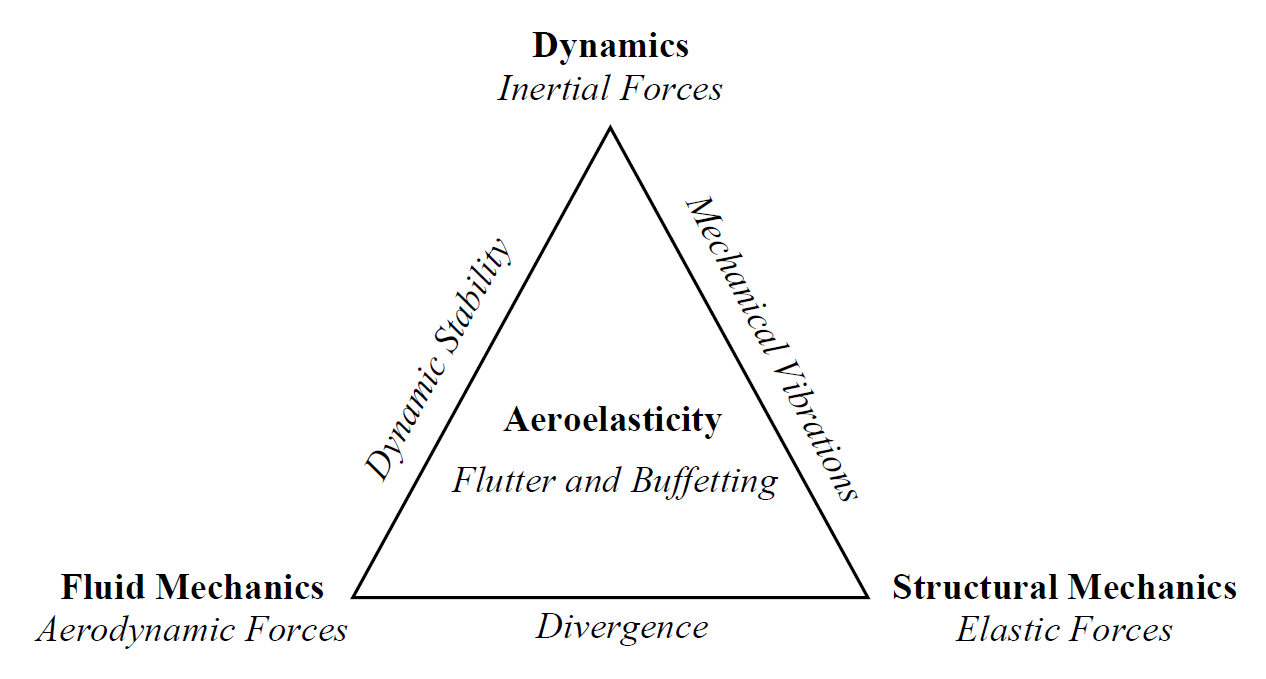
\includegraphics[width = .43\textwidth]{./Immagini/1_1.png}
\caption{Collar Triangle}
\label{fig:1_2}
\end{figure}
The interaction between these three forces can cause several undesirable phenomena like
divergence (static aeroelastic phenomenon), 
flutter (dynamic aeroelastic phenomenon), 
limit cycle oscillations (nonlinear
aeroelastic phenomenon), 
vortex shedding, buffeting, galloping
(unsteady aerodynamic phenomena) .
\subsection{Static aeroelasticity}
The interaction between the aerodynamic forces ans the elastic forces determine the static aeroelasticity phenomena. In this work we are principally interested to the aeroelastic coupling, the aerodynamic force induce on the wing a structural deformation, which modify the geometry of the wing, and then the aerodynamic forces. So to determinate correctly the aerodynamic forces it's necessary to determinate it whit an iterative process, where step by step the forces and the deformation are updated, until the convergence is reached.\\
A typical aeroelastic problem can be described by the following matrix equation:
\begin{equation*}
[M]\mathbf{\ddot{q}}+[C]\mathbf{\dot{q}}+[K]\mathbf{q}=\mathbf{F}(bs,\mathbf{q},\mathbf{\dot{q}},\mathbf{\ddot{q}},\mathbf{V},t,\omega)
\end{equation*}
where $[M]$ is the mass matrix, $[C]$ is the damping matrix, $[K]$ is the stiffness matrix, $\mathbf{\ddot{q}},\ \mathbf{\dot{q}},\ \mathbf{q}$ are the degree of freedom( and the first and second time derivatives), $\mathbf{\textbf{F}} $ is the aerodynamic force, $\mathbf{V}$ is the air speed, $t$ is the time, $\omega$ is the oscillation frequency and $bs$ indicate bodyshape, and define the join between the aerodynamic forces and the shape of the structure.\\
In a static model the equation became:
\begin{equation*}
[K]\mathbf{q}=\mathbf{F}(bs,\mathbf{q},\mathbf{V})
\end{equation*}
To understand how the problem involve the study of the typical aeroelastic section can be approached.
\subsubsection{Typical Aeroelastic Section}
The typical aeroelastic section consist in a model where the wing is assumed as a 2DoF system:
\begin{figure}[H]
	\centering
	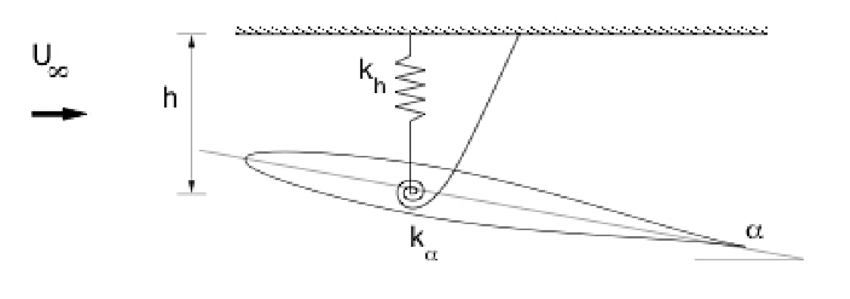
\includegraphics[width = 1\textwidth]{./Immagini/2_ala.png}
	\caption{Typical aeroelastic section}
	\label{fig:2_ala}
\end{figure}
The two DoF are the vertical translation $h$ and the rotation $\alpha$.
The stiffness is concentrated in the elastic axes, and is represented by two spring, one linear and one torsional, with respectively $K_h$ and $K{\alpha}$. Writing the equation of the rotation at the shear center we obtain:
\begin{equation*}
Wd+M{c.a.}+Le-K_{\alpha}\alpha=0
\end{equation*}
where $W$ is the weight, $d4$ the distance of the center of gravity and shear center, $e$ the distance of the aerodynamic center and shear center. Collecting the terms that depends of the rotation $\alpha$, we obtain:
\begin{equation*}
(K_{\theta}-qSC_{p,\alpha}e)\theta=M_0
\end{equation*}
where
\begin{equation*}
M_0=Wd+M{c.a.}+qSC_{p,{\alpha_0}}e
\end{equation*}
The term $K_{ae}=K_{\theta}-qSC_{p,\alpha}e$ is the aerodynamic stiffness. So in the moment when we consider the deformation of the wing the stiffness of the structure change, while the aerodynamic stiffness is coupled with the aerodynamic forces and structural displacement, so it's not possible to compute its value at the start of the process, from this an iterative method is used.\\
The divergence problem is caused from this pattern, in fact the aerodynamic stiffness reduce the stiffness of the structure, when the total stiffness reach the value of 0 the structure became instable.\\
In our work we don't consider the divergence problem, but just the aerodynamic coupling, solved by the MDA loop.